Los capículos previos dejan ver que la obtención de una imagen es un proceso complejo. Diversos sistemas actúan concertadamente para la obtención de la señal, que debe ser digitalizada y procesada para finalmente dar como resultado una imagen. En cada uno de los pasos involucrados existe el potencial de la introducción de errores, que repercuten negativamente en la imagen final. Se denomina \textit{artefacto} a cualquier anormalidad en la imagen derivada de un proceso fallido o erróneo durante la adquisición o procesamiento de la señal, que perturba la correcta interpretación del resultado. Mientras que algunos artefactos dominan la imagen y la convierten en inútil, otros son sutiles e interfieren poco con la interpretación clínica  de la imagen. Más peligrosos son los que pueden confundirse con anormalidades anatómicas. Es por eso que todo usuario de IRM debe conocer los diversos tipos de artefactos para poder identificarlos, distinguirlos de la anatomía en cuestión, y conocer  acciones  para minimizarlos. Este capítulo recopila los artefactos más frecuentes pero no pretende ser una lista exhaustiva. Cada técnica de IRM es susceptible a artefactos particulares, y es responsabilidad del usuario conocerlos.

Un aspecto particularmente interesante de los artefactos en IRM es que dejan ver la física y técnica detrás de la generación de la imagen. En otras palabras, los artefactos exageran la contribución de un proceso dentro de la cadena de generación de la imagen, y nos permiten entender mejor cómo funciona el sistema. Por otra parte, algunos artefactos pueden ser domados y convertidos en técnicas útiles.


\section{Artefactos derivados de los instrumentos}
Estos problemas se derivan de problemas técnicos, de manufactura, o de uso de los diferentes componentes del resonador (\textit{hardware}) o el cuarto en el que se encuentran.


\subsection{Artefacto de cremallera (\textit{zipper})}
Sucede cuando la antena receptora de la señal de RM recibe además una RF externa, no relacionada al tejido de interés. Habitualmente, el cuarto donde se alberga un resonador magnético dispone de una jaula de Faraday (todo el cuarto está envuelto en una malla de cobre) que impide que RF externas se propaguen dentro del cuarto. La jaula de Faraday limita las RF que habitualmente existen en el ambiente, que por sus frecuencias resultan relevante la radio FM y televisión (VHF). Defectos en la jaula de Faraday, o la presencia de un emisor de RF dentro del cuarto del resonador, serán fácilmente captados por la antena receptora, pues su amplitud es considerablemente mayor a la RF de resonancia. Al entrometerse en la recepción del eco, se traducen en líneas de ruido en la dirección de codificación de frecuencia.

\begin{figure}[htb]
 \begin{figg}
   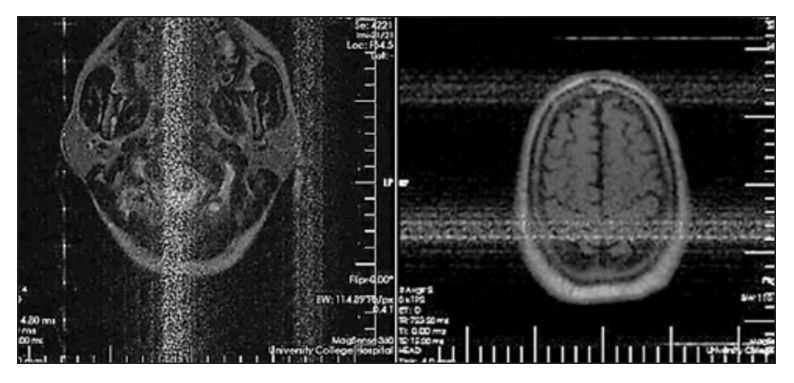
\includegraphics[width=0.7\textwidth]{artefacto_zipper}
   \caption{\figurapendiente  Tomada de \cite{ogbole2017brain}}
 \label{fig:artefacto_zipper}
 \end{figg}
\end{figure}



\subsection{Bandas de zebra}
Este artefacto tiene un origen similar al anterior, pero con una frecuencia constante, habitualmente causada por fallas de equipo eléctrico dentro del cuarto del resonador. Una vez que la RF espuria es captada por la antena, será mal interpretada como provenientes de la anatomía en estudio, e incluida dentro del \espaciok de acuerdo a su frecuencia y fase (Figura \ref{fig:artefacto_rfspike}).  Dado que cada celda de \espaciok representa la contribución de una orientación y frecuencia espacial, el artefacto se expresará como bandas que se repiten con cierta orientación y frecuencia, dependiendo de cuál celda de \espaciok resultó sobrevaluada. Este artefacto nos permite ver la relación entre imagen y \espaciok, y se minimiza mediante la eliminación de la RF externa.

\begin{figure}[htb]
 \begin{figg}
   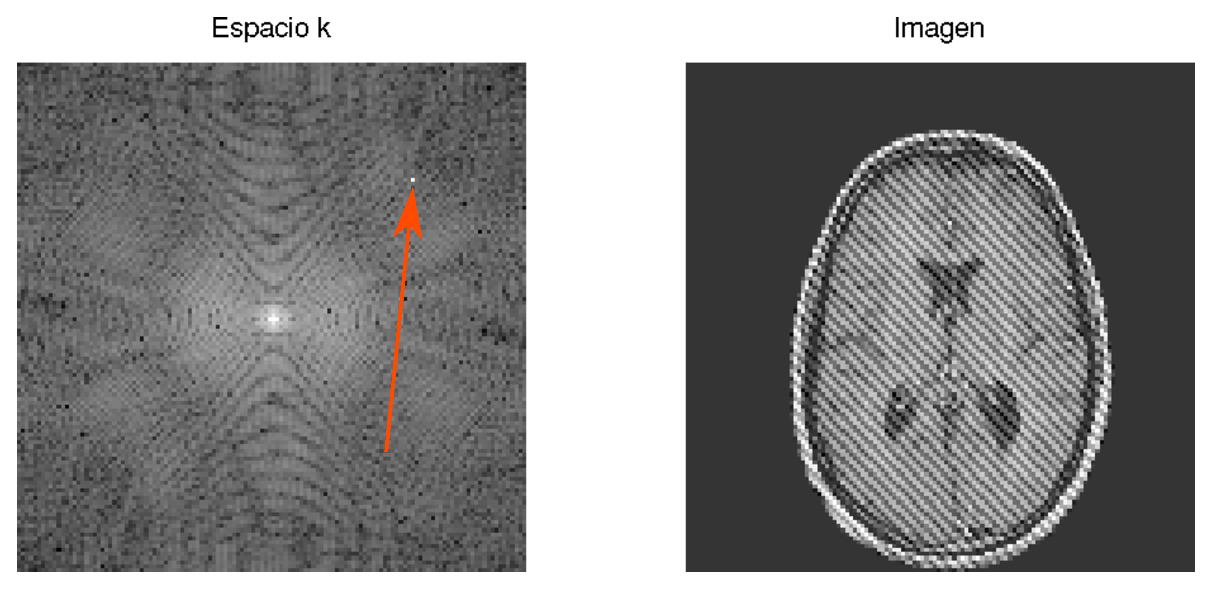
\includegraphics[width=0.7\textwidth]{artefacto_rfspike}
   \caption{\figurapendiente}
 \label{fig:artefacto_rfspike}
 \end{figg}
\end{figure}
 



\subsection{Efecto de Moiré}
Relacionado con el artefacto de enrollamiento, sucede más frecuentemente en imágenes con eco de gradiente y con FOV reducido. Comportamientos no lineales en los extremos de los gradientes codificadores provocan enrrollamiento de la señal, que provoca interferencia construcitiva/destructiva de las fases correspondientes, provocando bandas alternantes curvilíneas similares a las que se producen al mirar a través de dos mallas de mosquitero (Figure \ref{fig:artefacto_moire}). 


\begin{figure}[htb]
 \begin{figg}
   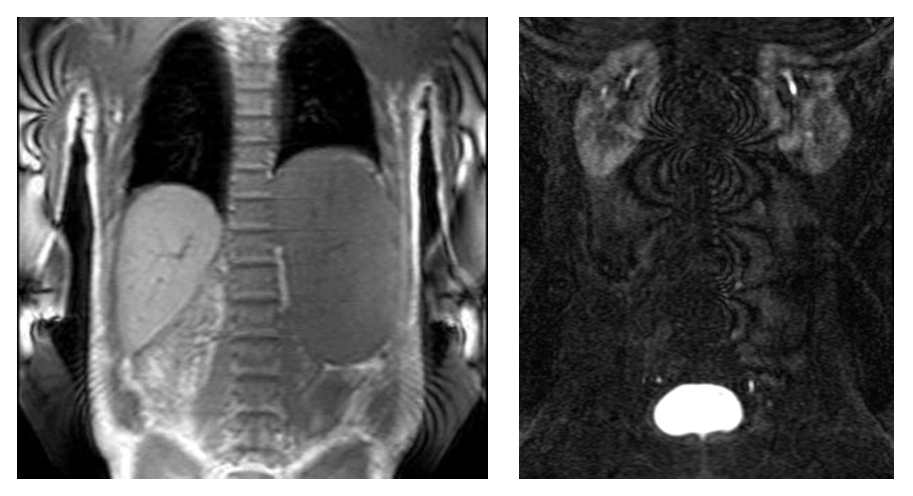
\includegraphics[width=0.7\textwidth]{artefacto_moire}
   \caption{\figurapendiente. Tomado de \url{https://radiopaedia.org/articles/moire-fringes-2}}
 \label{fig:artefacto_moire}
 \end{figg}
\end{figure}


\subsection{Saturación de RF}
La señal recibida debe digitalizarse antes de ser tratada mediante la transformada de Fourier. Una serie de amplificadores incrementan la magnitud de la señal antes de pasarla al convertidor analógico-digital (CAD). Si la amplificación de la señal es demasiada, el CAD se satura y se pierde el rango dinámico de la señal codificada. Esto se traduce una apariencia borrosa y variaciones de intensidad de la señal a lo largo de la imagen (Figura \ref{fig:artefacto_rfoverflow}).


\begin{figure}[htb]
 \begin{figg}
   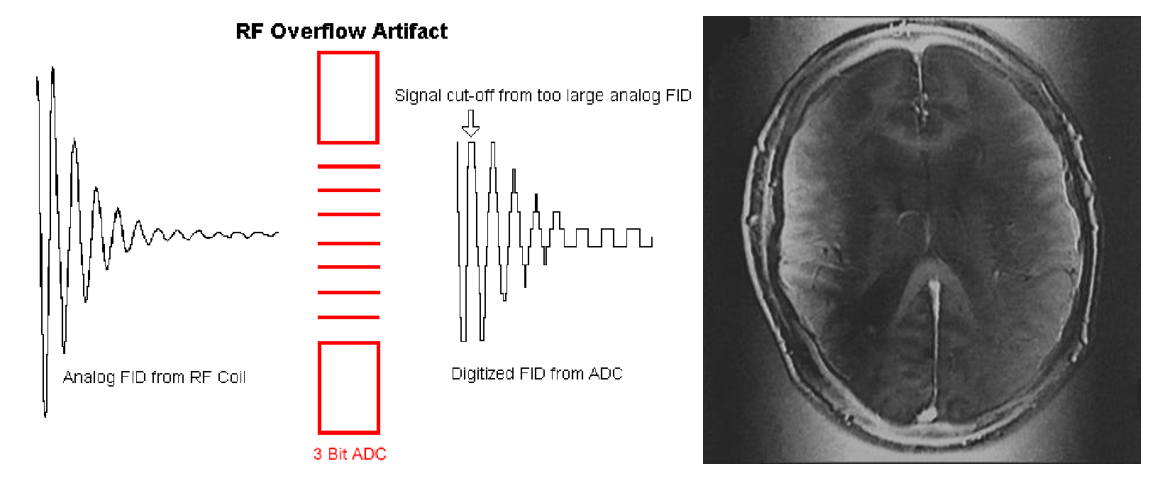
\includegraphics[width=0.7\textwidth]{artefacto_rfoverflow}
   \caption{\figurapendiente. Tomado de \url{https://radiopaedia.org/articles/moire-fringes-2}}
 \label{fig:artefacto_rfoverflow}
 \end{figg}
\end{figure}


\subsection{Inhomogeneidades de intensidad relacionados a la antena receptora}
La intensidad de la señal de RM disminuye en función de la distancia con respecto a la antena receptora (Figura \ref{fig:artefacto_inu}). Esto es idéntico a la manera en que una estación de radio se pierde mientras nos alejamos de la ciudad de donde se emite. Por lo tanto, se procura siempre que la antena receptora se acerque lo más posible a la anatomía a estudiar, razón por la cual existen muchos tipos de antena (para cráneo,  abdomen,  rodilla, etc). El efecto de pérdida de señal es sumamente notorio cuando utilizamos antenas de superficie, o en un solo lado de la anatomía. Ejemplo de ésto es la antena para ver columna vertebral que, aunque muy larga y colocada en contacto con la espalda del paciente, solo permite ver la columna y tejidos circundantes, pero el abdomen del paciente es prácticamente invisible. Otra característica de adquisiciones con inhomogeneidades de intensidad es que la relación señal/ruido es también inhomogénea, siendo más baja conforme se está más lejos de la antena.

Un punto a tener en consideración es que en las últimas dos décadas se han popularizado las antenas con múltiples canales. Estas funcionan como un arreglo de múltiples antenas con perfiles espaciales limitados que se sobrelapan. Cada elemento o canal ``ve'' una porción acotada de la anatomía con gran calidad, pero no logra captar señal de regiones más lejanas; éstas otras regiones son idealmente captadas por otros canales del arreglo de antenas. Por lo tanto, la inhomogeneidad de intensidad resultante es compleja y el ruido es espacialmente variable.

\begin{figure}[htb]
 \begin{figg}
   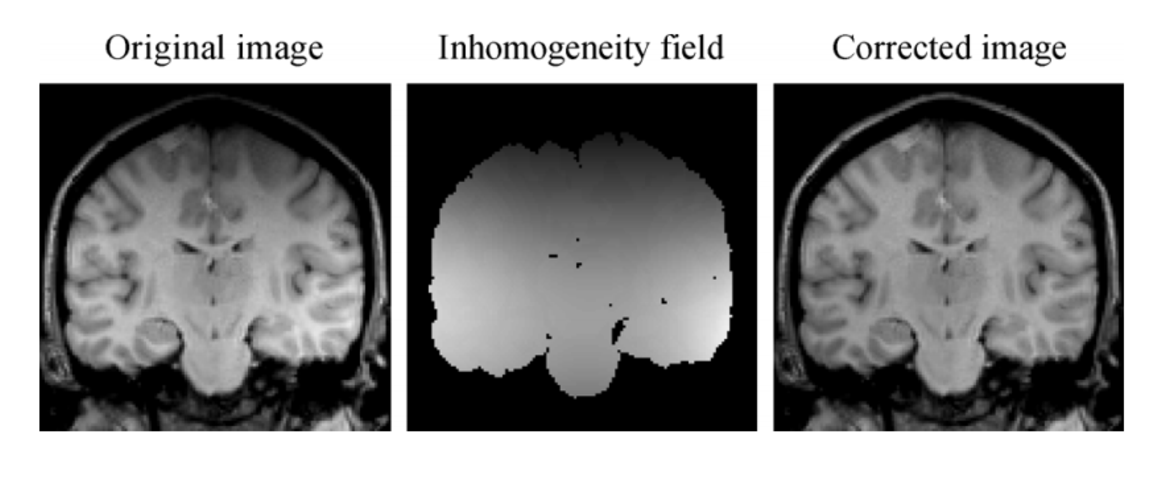
\includegraphics[width=0.7\textwidth]{artefacto_inu}
   \caption{\figurapendiente. Tomado de \cite{vovk_pernus_likar_2007}.}
 \label{fig:artefacto_inu}
 \end{figg}
\end{figure}




\subsection{Inhomogeneidades de \Bone}
Como se vió en el Capítulo \ref{chapter_secuencias}, el uso juicioso de pulsos de RF que provoquen desviaciones específicas del vector de magnetización (en combinación con el uso de gradientes del campo magnético) nos permite planear secuencias de pulsos que provoquen contrastes, resolución, y otras características específicas. Así, el usuario espera que al prescribir un pulso de RF de ciertas características (180\degrees, por ejemplo), el pulso se ejecute de manera homogénea a lo largo de toda la muestra. Esto último no siempre es así, debido a características de diseño de la antena emisora de RF. En muchas ocasiones, en un afán de adaptar la antena a la anatomía del paciente, la arquitectura resultante impide que el pulso de RF se transmita homogéneamente. En estas circunstancias, algunos tejidos experimentarán la modulación deseada (180\degrees en nuestro ejemplo), mientras que en otros tejidos será mayor o menor. Un pulso de 180\degrees, que podríamos usar para producir un eco, provocará el refasamiento del sistema de spins en mayor o menor medida, con cierta dependencia espacial, resultando en inhomogeneidades de intensidad espacialmente variables (Figura \ref{fig:artefacto_B1}). Una manera de minimizar este artefacto es el uso de dos antenas de forma secuencial: una antena (habitualmente circular, muy homogénea, y embebida en el resonador) se utiliza para emitir RF, mientras que una segunda antena (adaptada a la anatomía y colocada muy cerca del paciente) recibe la señal.


\begin{figure}[htb]
 \begin{figg}
   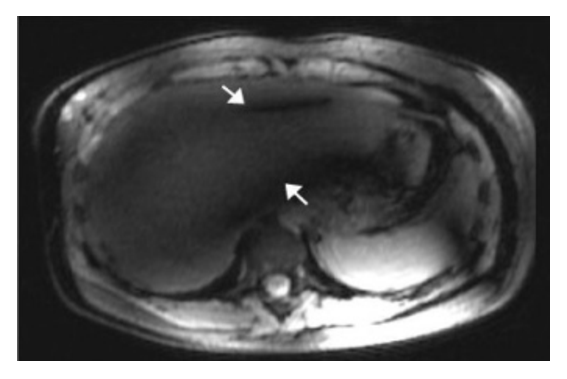
\includegraphics[width=0.7\textwidth]{artefacto_B1}
   \caption{\figurapendiente. Tomado de \cite{wu2014mitigating}.}
 \label{fig:artefacto_B1}
 \end{figg}
\end{figure}


\subsection{Inhomogeneidades geométricas}
La codificación espacial depende de una correcta interpretación de las frecuencias existentes en la señal recibida, con base en una ecuación lineal muy sencilla (página \pageref{eq_LarmorGradientes}). Se espera, entonces, que los gradientes del campo magnético que perturban los ejes $x$, $y$, y $z$, lo hagan de una manera perfectamente predecible y, sobre todo, lineal. Desviaciones de esta expectativa harán que ensambles de spins tengan frecuencias de precesión distintas a lo que deberían tener dada su localización espacial; posterior a la descomposición espectral mediante la transformada de Fourier, las frecuencias anómalas serán interpretadas como una localización espacial errónea (Figura \ref{fig:artefacto_Ginhomo}). Las no-linearidades de los gradientes son casi inevitables en sus extremos, por lo que los fabricantes informan los FOVs máximos posibles en cada dimensión. Una falla de linearidad en las partes más centrales del gradiente es indicadora de una falla de manufactura.

\begin{figure}[htb]
 \begin{figg}
   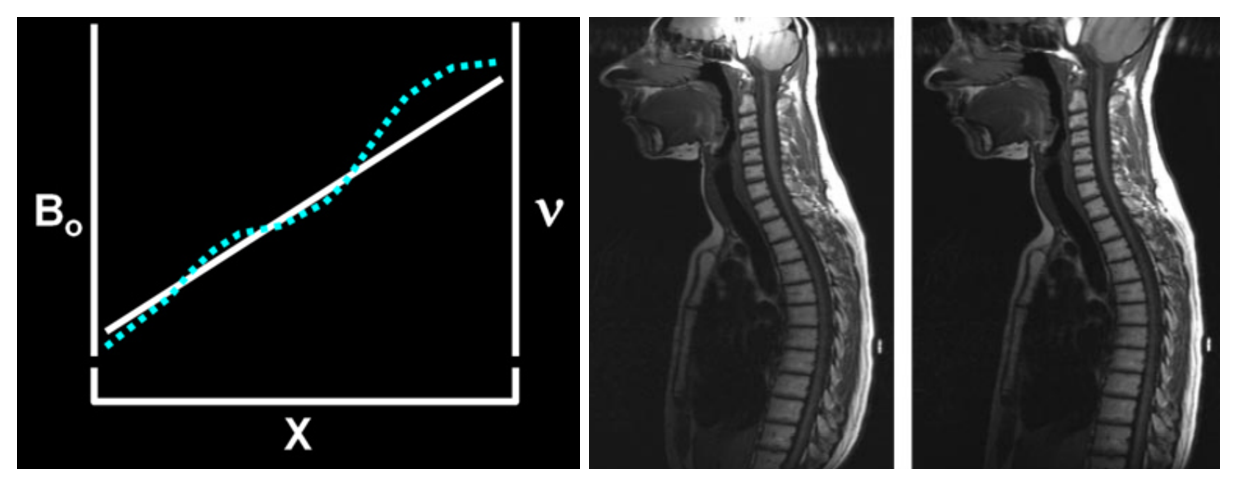
\includegraphics[width=0.7\textwidth]{artefacto_Ginhomo}
   \caption{\figurapendiente. }
 \label{fig:artefacto_Ginhomo}
 \end{figg}
\end{figure}




\section{Artefactos asociados a la transformada de Fourier}
\subsection{Anillos de Gibbs}
Recordemos que una imagen es resultado de la transformada de Fourier (2D) del \espaciok, y que en teoría cualquier señal puede ser construida a partir de la suma de un número infinito de frecuencias puras. En el mundo real, sin embargo, es imposible muestrear un número infinito de frecuencias en el \espaciok, por lo que su transformación en una imagen  es meramente una aproximación \cite{gallagher2008fourier}. Tener que truncar las frecuencias en un \espaciok finito tiene sus consecuencias, que son visibles principalmente en los bordes de estructuras anatómicas, donde la intensidad de la imagen cambia abruptamente de un voxel a otro. En términos de señales, consideramos estas regions como de ``alta frecuencia'', codificadas en la periferia del \espaciok (Capítulo \ref{chapter_espacial}). Para comprender por qué un borde anatómico es una región de alta frecuencia, imaginemos que queremos dibujar un escalón de perfil. Es decir, un ``dibujo'' simple, en una dimensión, donde la altura representa la amplitud de la señal, y el eje $x$ el espacio. Ahora, dibujemos ese mismo escalón, pero usando la transforamada de Fourier. Agregaremos una primer frecuencia base, que sube y baja (como una función seno), con lo que lograremos algo que parece un escalón, pero demasiado curvo como para ser considerado seguro. Así que agregamos una frecuencia más alta, sumándose a la primera, con lo que producimos una nueva forma que respeta la forma del escalón, pero con muchos surcos. Una frecuencia más es agregada, y se van afinando los surcos, otra, y otra, y así sucesivamente, con lo que vamos viendo cómo nuestro escalón se va haciendo cada vez más recto, y las ondulaciones (los surcos) cada vez menos pronunciadas. Para un escalón perfectamente cuadrado deberíamos entonces agregar un número infinito de frecuencias. Como no es posible, dejamos de agregar frecuencias más altas (llegamos a los bordes del \espaciok y no podemos agregar más), dándonos como resultado algo que parece un escalón, pero que tiene poquitos holanes. Estos holanes (o faralás) son el artefacto de Gibbs (Figura \ref{fig:artefacto_gibbs}). En una imagen de cráneo, por ejemplo, los bordes más evidentes son en la frontera entre la corteza y el líquido cefalorraquídeo. Los anillos de Gibbs se aprecian como repeticiones fantasmales de dicha frontera dentro de la corteza. El nombre del artefacto se debe a J. Willard Gibbs, quien describió algunos de los límites prácticos de la transformada de Fourier en 1899.

Este artefacto sucede en las direcciones de codificación en frecuencia y fase; como habitualmente se muestrea incluso menos la codificación en fase (porque consume tiempo TR), el artefacto suele ser más notorio en dicha dirección. Aunque no puede ser totalmente eliminado, puede minimizarse aumentando la resolución y el número de renglones del \espaciok (con lo que aumenta la tasa de muestreo), o utilizando técnicas de post-proceso que suavizan el artefacto al filtrar las señales obtenidas. 

\begin{figure}[htb]
 \begin{figg}
   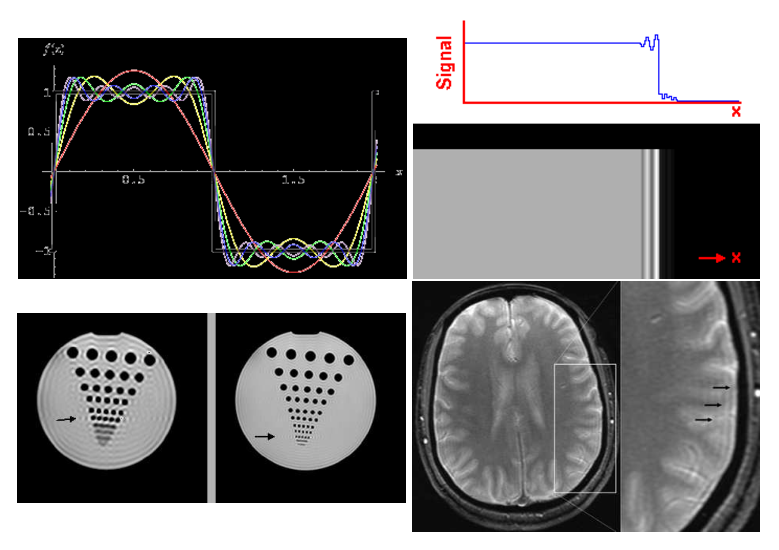
\includegraphics[width=0.7\textwidth]{artefacto_gibbs}
   \caption{\figurapendiente. Tomado de \cite{gallagher2008fourier} y \url{http://www.cis.rit.edu/htbooks/mri/}.}
 \label{fig:artefacto_gibbs}
 \end{figg}
\end{figure}



\subsection{Enrollamiento de la imagen (\textit{alias})}
Las señales analógicas capturadas por la antena receptora son digitalizadas y vertidas en el \espaciok. La digitalización implica convertir una señal continua en una discreta, teniendo un punto de información (muestra) cada cierto tiempo. En teoría de señales se dice que una señal se enrrolla (presenta alias) cuando la tasa de muestreo es insuficiente para capturar la forma de la señal analógica original. Este fenómeno es muy notorio en escenas cinematográficas donde se observan hélices de helicópteros o las ruedas de una bicicleta, dando la impresión de que giran lentamente, o incluso en reversa. El término \textit{alias} es, entonces, adecuado, porque una frecuencia representa en realidad a otra; el problema es que este enmascaramiento es irreversible.  En términos de imagen, el enrollamiento se observa como una región anatómica colocada espacialmente en el sitio opuesto de la imagen, como si se hubiera forrado un cilindro con la imagen (enrollamiento), que luego se hubiera cortado en el sitio incorrecto (Figura \ref{fig:artefacto_alias}).

\begin{figure}[htb]
 \begin{figg}
   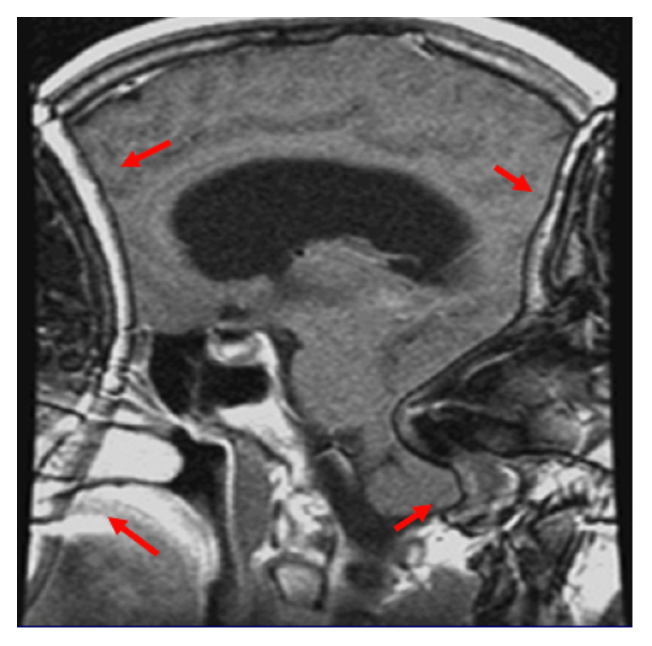
\includegraphics[width=0.7\textwidth]{artefacto_alias}
   \caption{\figurapendiente }
 \label{fig:artefacto_alias}
 \end{figg}
\end{figure}


Para cualquier señal que uno desee digitalizar evitando el fenómeno de alias, la tasa de muestre debe ser al menos el doble de la frecuencia más alta contenida en la señal analógica, algo conocido como el \textit{criterio de Nyquist}\index{Nyquist}. En imagen podemos saber \textit{a priori} cuál será la frecuencia más alta que necesitamos digitalizar, pues provendrá de la orilla del FOV utilizado. Recordemos que la localización espacial se codifica mediante modificaciones de la frecuencia de precesión (y por consiguiente de la fase) a través de gradientes del campo magnético, y la ecuación \ref{eq_LarmorGradientes} (Capítulo \ref{chapter_espacial}) nos permite deducir la frecuencia máxima que se logrará mediante la aplicación del gradiente en la máxima amplitud que prescribiremos. Sin embargo, los gradientes ejercen su efecto incluso más allá del FOV que utilizamos, por lo que cualquier tejido que se encuentre más allá del borde del FOV emitirá señal a cierta (alta) frecuencia, que será digitalizada incorrectamente (sub-muestreada). La frecuencia enrollada codificará entonces incorrectamente la posición del espacio del tejido que emitió la alta frecuencia, y la anatomía aparecerá en un sitio inadecuado en la imagen.

La manera más sencilla de evitar el enrollamiento de la imagen es mediante el uso de un FOV suficientemente amplio como para que no exista anatomía más allá de sus bordes. Esto es trivial en algunas regiones anatómicas y en ciertos cortes (por ejemplo un corte axial de cráneo), pero imposible en otras regiones del cuerpo. El enrollamiento de la imagen puede suceder en los ejes codificados mediante frecuencia y fase, pero es en esta última donde suele expresarse más comunmente. Esto se debe a que es fácil sobre-muestrear una señal en la codificación por frecuencia (simplemente se aumenta la tasa de muestreo del digitalizador, con la única consecuencia siendo el incremento de datos almacenados), mientras que el sobre-muestreo de la dimensión codificada por fase implicaría llenar más líneas de \espaciok, por los que habría que pagar un tiempo mayor de adquisición (un TR por cada línea de \espaciok en secuencias no aceleradas). 


\section{Artefactos derivados por parámetros de adquisición}
\subsection{Contaminación cruzada de rebanadas}
La excitación selectiva de una rebanada de tejido se logra mediante la combinación de un gradiente magnético y un pulso de RF (Capítulo \ref{chapter_espacial}). Como se describió en la sección dedicada a los anillos de Gibbs, la transformada de Fourier de un número finito de frecuencias no es idéntica a la señal analógica original. Para obtener una rebanada perfectamente definida en sus bordes tendríamos entonces que incluir un número infitito de frecuencias (con distintas amplitudes) en nuestro pulso de RF. En la realidad, se incluyen las frecuencias ubicadas en cierto rango (ancho de banda) que coincide con las frecuencias de precesión de la región que queremos excitar selectivamente. Nuestra rebanada entonces no tiene bordes definidos, como si se hubieran hecho con bisturí, sino bordes flojos y difuminados (Figura \ref{fig:artefacto_slice}). El artefacto de contaminación cruzada de rebanadas o sobrelape de rebanadas (\textit{slice cross-talk, slice overlap}, en inglés) sucede cuando tenemos rebanadas contiguas (Capítulo \ref{chapter_secuencias}): la excitación de una rebanada excita también algunos spins de la rebanada contigua y para cuando se excita selectivamente la segunda, dichos spins se encuentran excitados y no desarrollan el contraste deseado (estando incluso saturados, con lo que no logran emitir señal alguna). En frecuente que el artefacto no sea muy notorio, a no ser que se haga una reconstrucción de las imágenes en un plano ortogonal al de adquisición (por ejemplo, si las imágenes se adquirieron en plano axial, el artefacto será visible en los planos coronal y sagital como bandas alternantes de alta y baja intensidad). Cuando las adquisiciones son oblicuas con intersecciones entre ellas (como sucede habitualmente cuando se adquieren imágenes axiales de la columna vertebral, que presenta ondulaciones a lo largo de su eje supero-inferior), la contaminación entre rebanadas sucede justo en sus regiones de intersección.

\begin{figure}[htb]
 \begin{figg}
   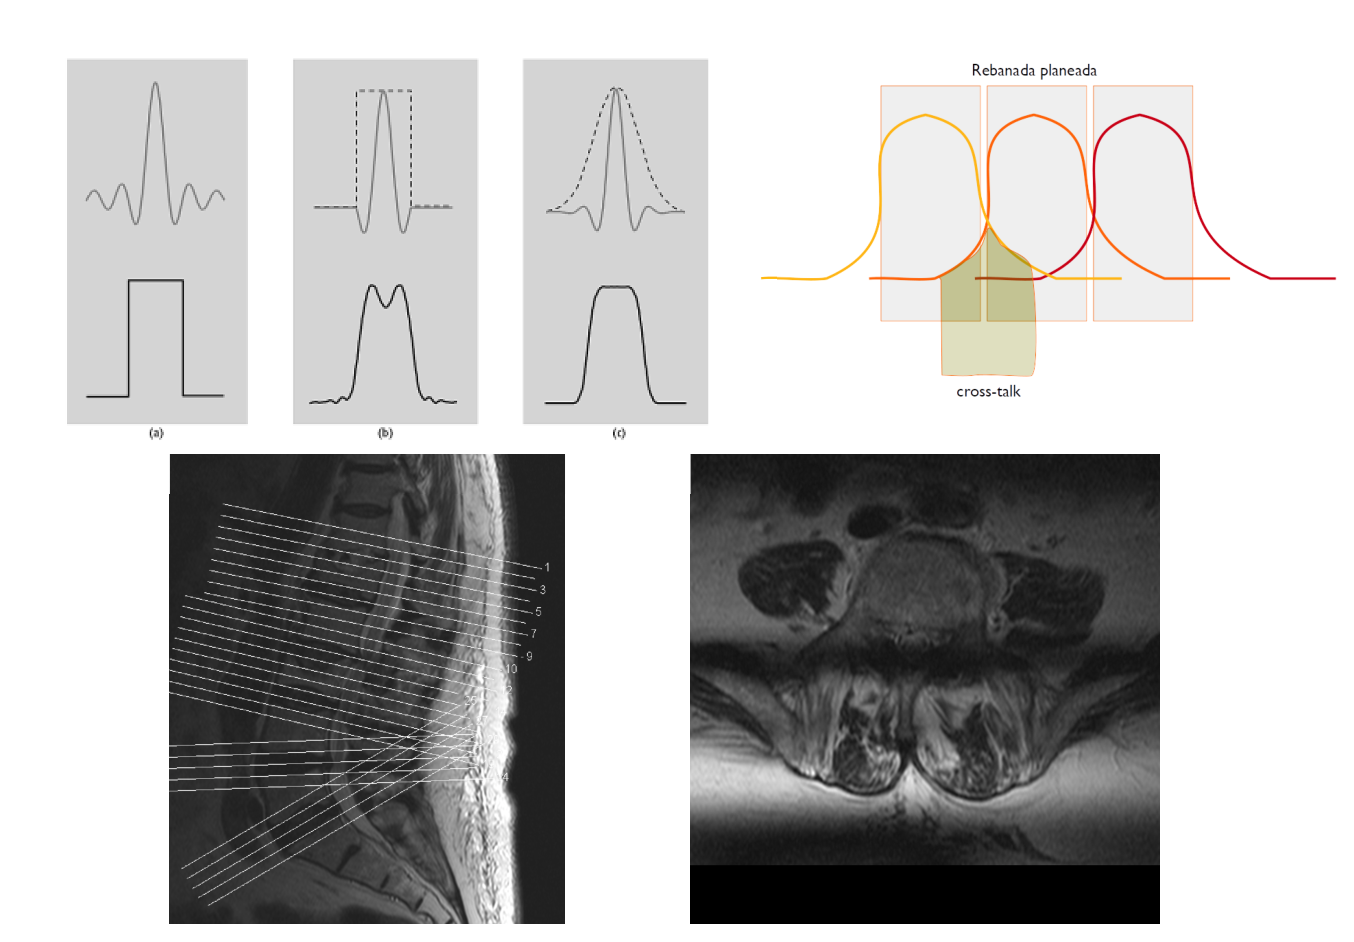
\includegraphics[width=0.7\textwidth]{artefacto_slice}
   \caption{\figurapendiente Tomado de \url{https://radiopaedia.org}}
 \label{fig:artefacto_slice}
 \end{figg}
\end{figure}


Existen varias estrategias para minimizar este artefacto. La primera es el uso juicioso del ancho de banda requerido para la excitación selectiva. Así, la aproximación más cercana a un pulso cuadrado de RF (rebanada bien delimitada) es un pulso de RF modulado mediante una función $\mathrm{sinc}(x)=\frac{\sin(x)}{x}$. Aún así, el pulso tendrá artefactos de Gibbs, por lo que la solución es incompleta. La segunda estrategia es dejar un espacio o brecha entre rebanadas (\textit{inter-slice gap}, en inglés), de manera que la excitación de una rebanada no logre contaminar a la siguiente. Lógicamente, esto puede acarrear problemas diagnósticos si una pequeña lesión se encuentra precisamente en una de estas brechas. La tercera estrategia es cambiar el orden de excitación de las rebanadas, dejando de ser una excitación secuencial de rebanadas contiguas, a una excitación donde, por ejemplo, se exciten primero todas las rebanadas con número impar, y luego todas las rebanadas pares, considerando que para cuando hayamos excitado la última rebanada del primer conjunto, ya se habrá relajado el tejido que se excitó artificiosamente en la primera rebanada a adquirir del segundo conjunto. A una adquisición de rebanadas así se le conoce como intercalada (\textit{interleaved}, en inglés).


\subsection{Efecto de volumen parcial}
Los voxeles, unidades mínimas de la imagen, son cuboides cuyas dimensiones están determinadas por el grosor de la rebanada y la relación entre FOV y el tamaño de la matriz del \espaciok. Cada voxel solo puede adquirir un solo valor de intensidad.  Por su forma y dimensiones, es habitual que más de un tipo de tejido exista dentro de un voxel determinado, potencialmente con características magnéticas muy distintas entre ellos. Cuando esta mezcla de tejidos intra-voxel sucede, el valor de intensidad del mismo será el promedio de las señales que produce cada tejido, pesado a la concentración correspondiente de cada uno de ellos (\ref{fig:artefacto_volumenparcial}). Como es de esperarse, el efecto de volumen parcial es mayor cuando se utilizan voxeles de gran tamaño, y se minimiza (pero nunca se puede eliminar por completo) cuando se usan imágenes con alta resolución. Es importante recordar que el efecto de volumen parcial puede suceder por la mezcla de tejidos en el espesor de la rebanada (es común, en adquisiciones de dos dimensiones, que el grosor de la rebanada sea considerablemente mayor a la resolución en el plano de la imagen).

\begin{figure}[htb]
 \begin{figg}
   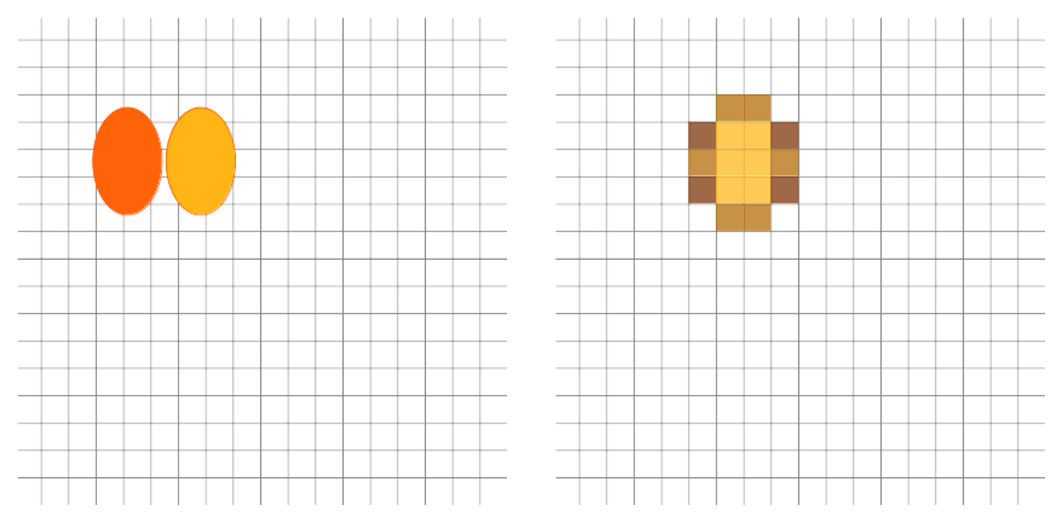
\includegraphics[width=0.7\textwidth]{artefacto_volumenparcial}
   \caption{\figurapendiente}
 \label{fig:artefacto_volumenparcial}
 \end{figg}
\end{figure}

\section{Artefactos producidos por movimiento}
\subsection{Movimiento del paciente}
Quizás el artefacto más sencillo de entender, sucede cuando la anatomía se mueve entre la adquisición de distintas líneas de \espaciok (entre TRs). Este artefacto hace notoria la ausencia de relación 1:1 entre la imagen y el \espaciok correspondiente (página \pageref{sec:espaciok}), así como el hecho de que la transformada de Fourier de una sola línea del \espaciok contiene suficiente información para dibujar algo que parece el objeto original (Figura \ref{fig:proyeccionFrecuencia}). Así, al realizarse la transformada de Fourier se verán ``fantasmas'' de la anatomía original en una localización espacial distintas (Figura \ref{artefacto_movimiento}).

\begin{figure}[htb]
 \begin{figg}
   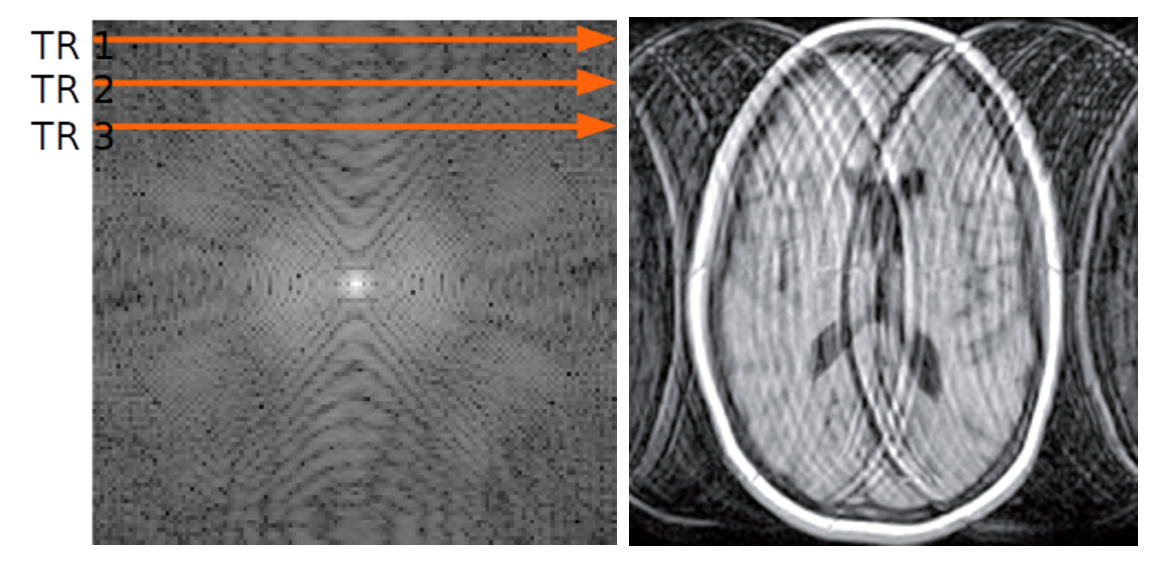
\includegraphics[width=0.7\textwidth]{artefacto_movimiento.eps}
   \caption{El voluntario se ha movido entre distintos TRs a lo largo del llenado del \espaciok (izquierda). La imagen resultante muestra varias copias movidas de la anatomía original (derecha).}
 \label{fig:artefacto_movimiento}
 \end{figg}
\end{figure}
 

Eliminar este artefacto puede ser tan fácil como difícil, dependiendo de la fuente de movimiento. Por ejemplo, en la obtención de imágenes de cráneo, se debe pedir al voluntario que no se mueva, y pueden colocarse almohadillas alrededor de la cabeza para limitar el movimiento involuntario. Sin embargo, es más difícil lograr la ausencia de movimiento cuando uno realiza, por ejemplo, imágenes de tórax. Puede solicitarse un periodo de apnea (abstenerse de respirar) mientras se obtienen unas líneas de \espaciok, e ir obteniéndolas todas a lo largo de varios periodos de apnea. Las y los lectores imaginarán que aquéllos pacientes a quienes se solicita una resonancia de tórax con fines diagnóstico difícilmente podrán abstenerse de respirar por mucho tiempo. Otras fuentes de movimiento son totalmente involuntarias, como el latido del corazón o, peor aún, el movimiento peristáltico de las asas intestinales. Sin embargo, existen astutas estrategias que utilizan señales periféricas para sincronizar el movimiento de la anatomía con la adquisición progresiva de líneas de \espaciok. Por ejemplo, es posible utilizar un sensor para monitorizar el ciclo  cardiaco, identificando una característica del registro (periodo QRS en el electrocardiograma, por ejemplo) para iniciar la adquisición de tantas líneas de \espaciok sean posibles durante la diástole cardiaca (Figura \ref{fig:artefacto_trigger}). Lo anterior aplica de manera similar a la monitorización del ciclo respiratorio. Con estas estrategias, el tiempo de adquisición de la imagen se ve influido por la frecuencia del ciclo fisiológico en cuestión. Llevando esta idea un paso más adelante, es posible adquirir constantemente datos, durante cualquier momento del ciclo fisiológico (cardiaco, por ejemplo), y grabar de manera paralela la señal de resonancia, y la del electrocardiograma. \textit{A posteriori}, se reúnen todas las líneas de \espaciok recabadas en cada momento del ciclo cardiaco de acuerdo a la señal del monitor cardiaco, armando distintas imágenes correspondientes a cada uno de los periodos del ciclo. De esta forma, pueden generarse imágenes pseudo-dinámicas, donde se puede observar un ciclo cardiaco completo a manera de película. Nótese que nunca se obtuvo ``una imagen'' de cada parte del ciclo cardiaco, sino que cada parte se armó mediante fragmentos de distintos latidos a lo largo del tiempo.



 \begin{figure}[htb]
 \begin{figg}
   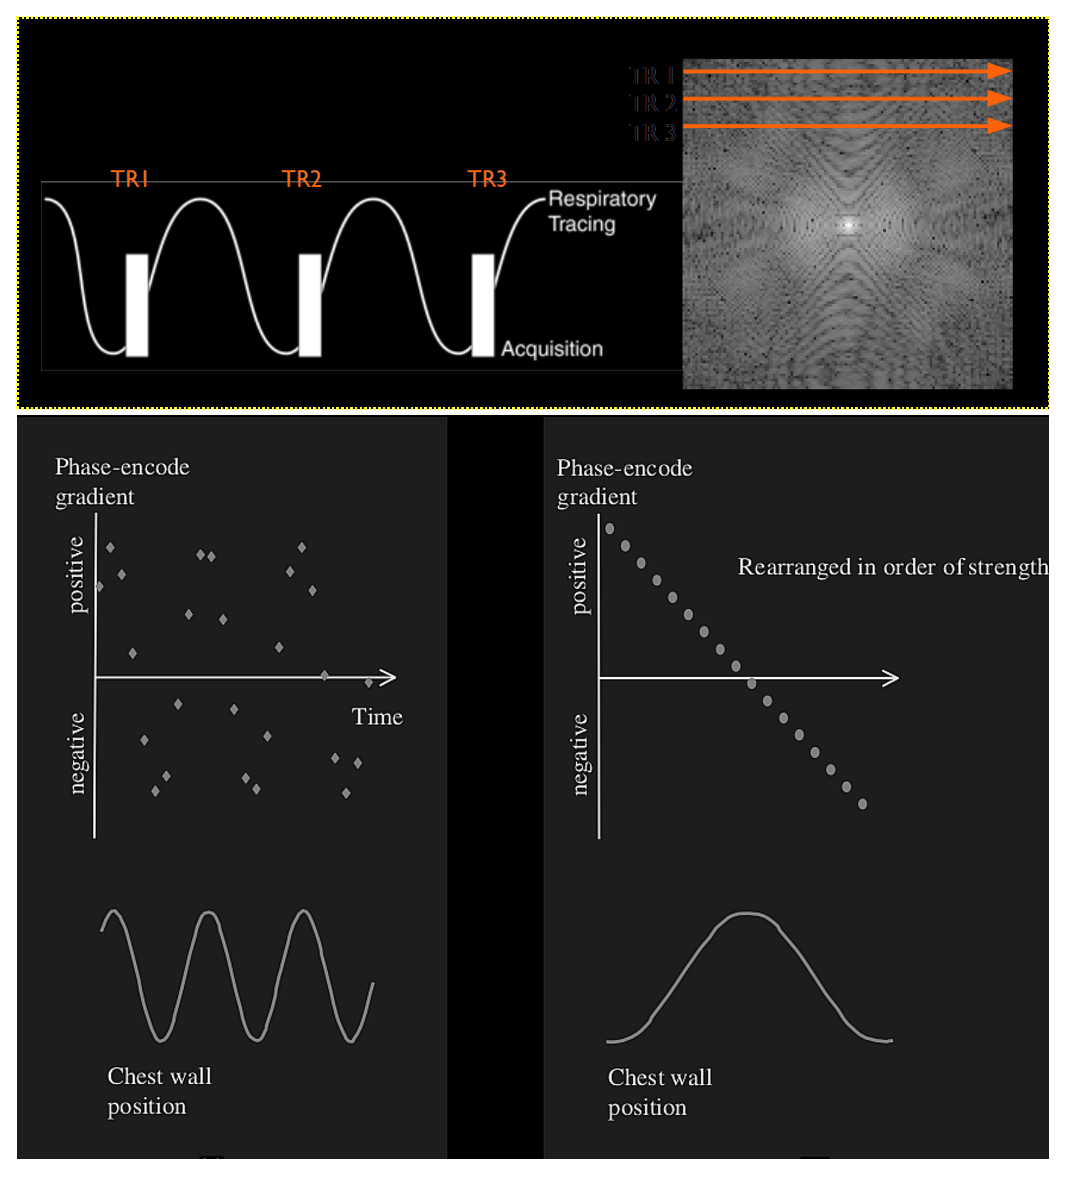
\includegraphics[width=0.7\textwidth]{artefacto_trigger}
   \caption{\figurapendiente}
 \label{fig:artefacto_trigger}
 \end{figg}
\end{figure}
 

\subsection{Movimiento por flujo sanguíneo}
El movimiento de la sangre a través de una rebanada de IRM tiene consecuencias interesantes que dependen del tipo de imagen que se está realizando, y la manera en que el vaso sanguíneo incide en el plano de la imagen. 

En imágenes adquiridas mediante eco de spin, donde se requiere un pulso excitador ($\alpha$\degrees) y un pulso para reenfocar los spins (180\degrees), es necesario que el tejido reciba ambos pulsos de RF para poder emitir señal. Si un vaso sanguíneo atraviesa perpendicularmente a una rebanada de IRM, la sangre presente en el espesor de la rebanada recibirá el pulso excitador pero (si el flujo es suficientemente rápido) abandonará a la rebanada antes de recibir el pulso de 180\degrees (Figura \ref{fig:artefacto_flow}). Esto ocasionará que esa parte de la imagen no brinde señal, con lo que el vaso se apreciará vacío (obscuro, hipointenso). Si el vaso sanguíneo corre paralelo al plano de la rebanada, la sangre recibirá tanto el pulso excitador como el de reenfoque, con lo que el vaso se apreciará lleno (brillante, hiperintenso).

\begin{figure}[htb]
 \begin{figg}
   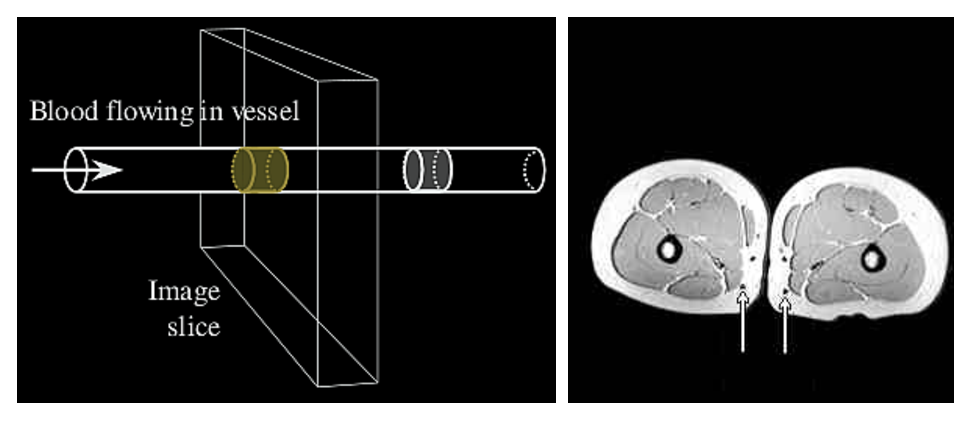
\includegraphics[width=0.7\textwidth]{artefacto_flow}
   \caption{\figurapendiente}
 \label{fig:artefacto_flow}
 \end{figg}
\end{figure}

En imágenes con TRs muy cortos, el tejido en toda la rebanada se encuentra parcialmente excitado (incluso saturado) entre pulsos $\alpha$ sucesivos. Sin embargo, cuando entra sangre a la rebanada, ésta no ha experimentado pulsos excitatorios previos, con lo que es capaz de aportar señal. Este fenómeno se conoce como ``tiempo de vuelo'' (\textit{time-of-flight} \index{TOF, time of flight}) y forma la base de uno de los métodos para visualizar vasos sanguíneos (angiografía, Capítulo \ref{chapter_angio}). 

Mediante secuencias multi-rebanada mediante eco de gradiente, es posible que la sangre sufra excitación en una rebanada, y exprese su señal en otras rebanadas, ya que la aplicación del gradiente generador del eco (y su respectiva inversión) no es selectivo de rebanada. 




\section{Artefactos por modulación local del campo magnético}
\subsection{Susceptibilidad magnética}
La susceptibilidad magnética ($\chi$) es la capacidad de un material de ser magnetizado por un campo magnético. Los materiales paramagnéticos ($\chi>0$) se alinean a favor del campo magnético, incrementando el campo magnético a su alrededor, mientras que los materiales diamagnéticos ($\chi<0$) se alinean en contra del campo magnético, disminuyendo su intensidad localmente. Los materiales ferromagnéticos tienen por sí mismos la capacidad de producir un campo magnético.

La frecuencia de precesión es el pilar de toda codificación espacial y de generación de contraste. Por lo tanto, la presencia de materiales paramagnéticos y diamagnéticos en o alrededor del tejido tendrán la capacidad de modular la señal generada y su codificación. Por ejemplo, cuerpos extraños con materiales que puedan modular el campo magnético local lograrán alterar la codificación espacial del propio objeto, y de los tejidos que le circundan (Figura \ref{fig:artefacto_brackets}). Esto es notorio alrededor de prótesis metálicas que, aunque están fabricadas actualmente mediante materiales seguros para el paciente, presentan suficiente cantidad de materiales que afectan el campo magnético de manera local. También se observa pérdida de señal y mala localización espacial de los elementos orales en pacientes con trabajo dental (brackets). 

La magnitud de los artefactos producidos por susceptibilidad magnética son directamente proporcionales a \Bzero, y son más acentuados en secuencias con TE largos (los spins tendrán más tiempo para desfasarse entre ellos). El uso de ancho de banda amplio minimiza el artefacto (aunque incrementa por sí mismo la cantidad de ruido en la imagen).


\begin{figure}[htb]
 \begin{figg}
   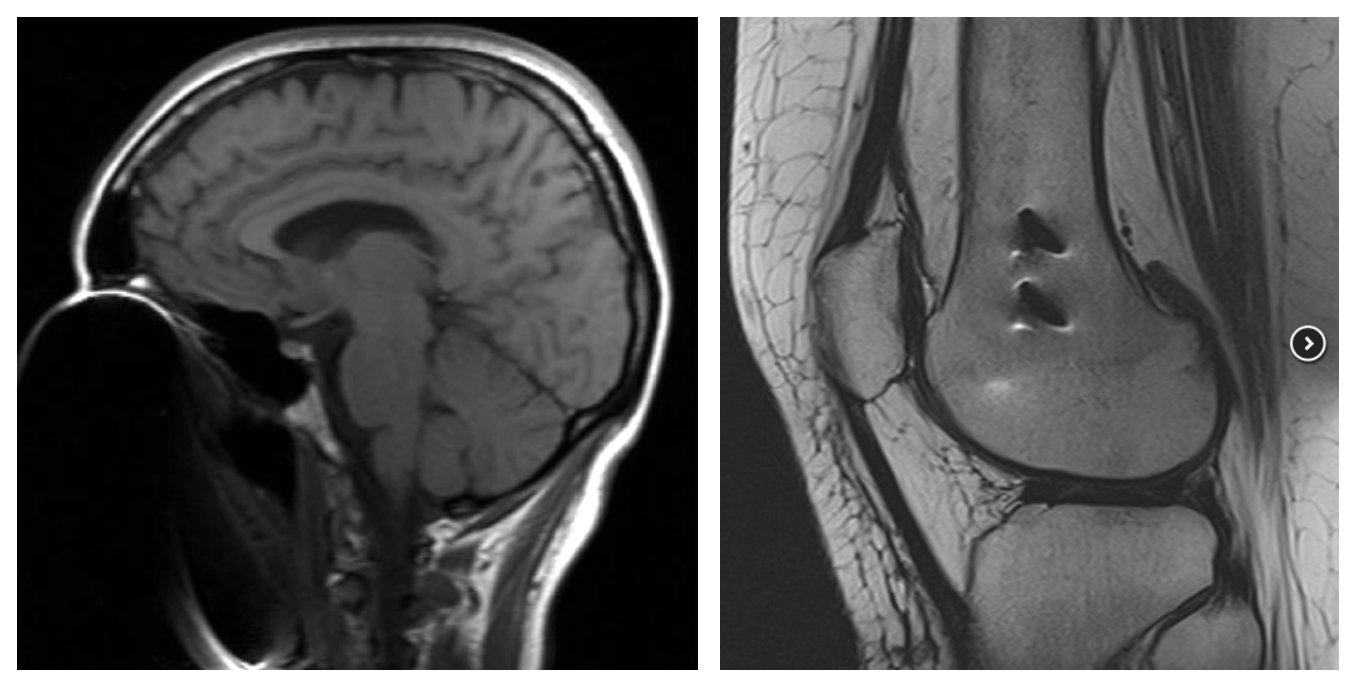
\includegraphics[width=0.7\textwidth]{artefacto_brackets}
   \caption{\figurapendiente}
 \label{fig:artefacto_brackets}
 \end{figg}
\end{figure}


Algunos artefactos por susceptibilidad magnética se producen incluso en ausencia de cuerpos extraños. Por ejemplo, los productos de descomposición de la hemoglobina exponen más al Fe presente en el grupo heme, lo que produce una mayor inhomogeneidad de \Bzero a su alrededor. Esto permite la etapificación de un evento hemorrágico y la visualización de algunas malformaciones arteriovenosas. 

La proximidad de materiales con distinta $\chi$ provoca alteraciones severas de \Bzero a nivel local que, en conjunción con imágenes con TE largo, pueden provocar molestos artefactos de imagen. Esto es común en imágenes ecoplanares (EPI) utilizadas para resonancia magnética funcional e imágenes sensibles a difusión, en las que la proximidad aire/tejido alrededor de los senos paranasales provoca áreas con pérdida de señal (Figura \ref{fig:artefacto_susceptibility_EPI}; Sección \ref{sec:ArtefactosDWI}). La mayoría de los tejidos son débilmente diamagnéticos, mientras que el aire (por la presencia del Oxígeno) es ligeramente paramagnético. Estos artefactos se minimizan mediante el uso de adquisiciones ecoplanares segmentadas (más de 1 TR por imagen), y métodos alternativos de llenado del \espaciok que disminuyen el TE efectivo. 


\begin{figure}[htb]
 \begin{figg}
   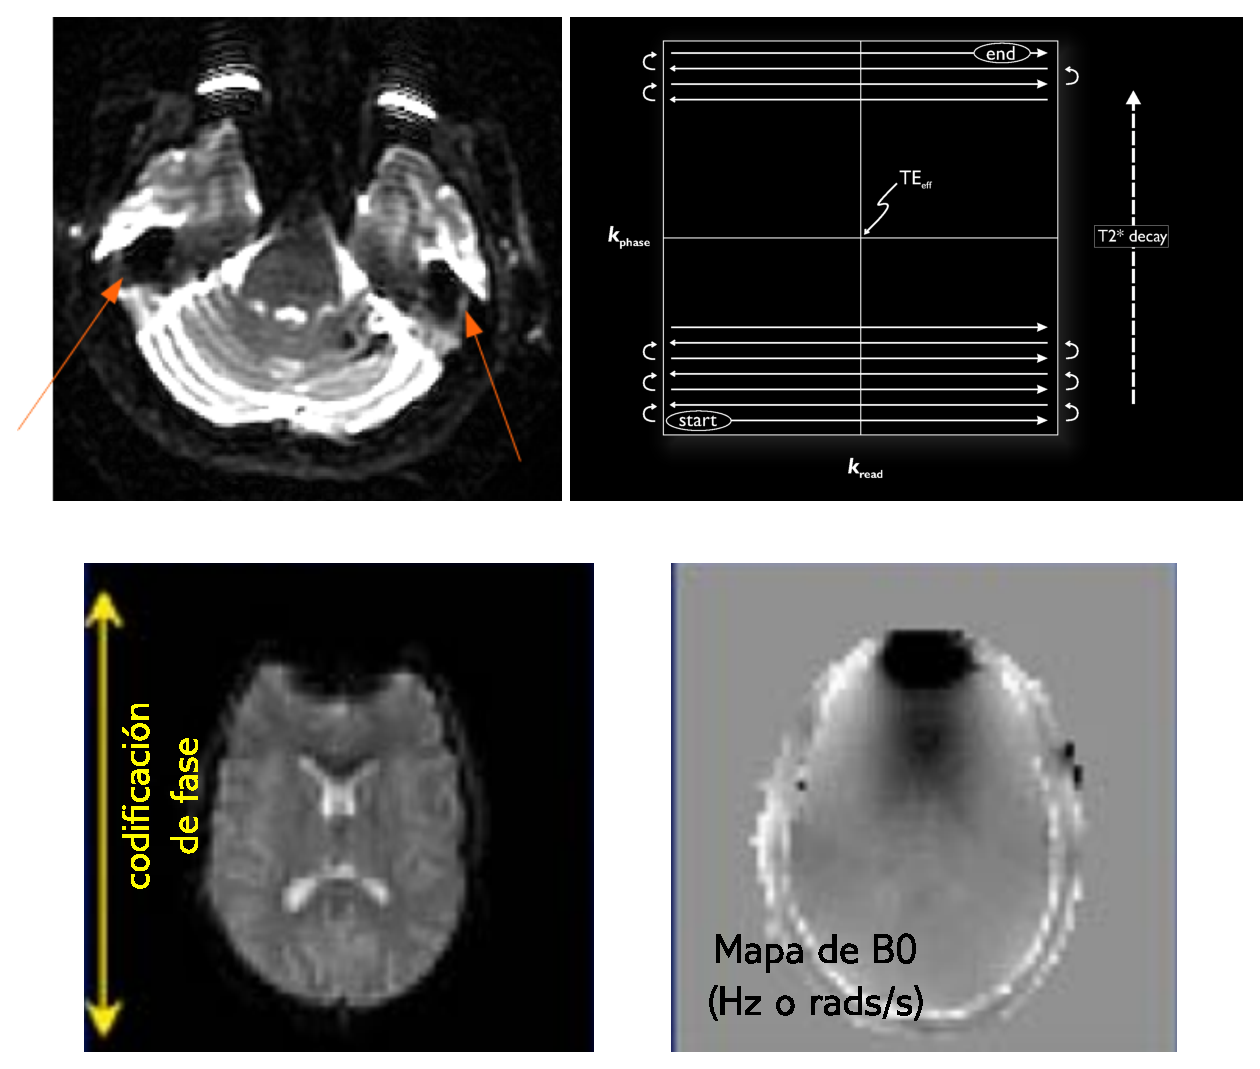
\includegraphics[width=0.7\textwidth]{artefacto_susceptibility_EPI}
   \caption{\figurapendiente}
 \label{fig:artefacto_susceptibility_EPI}
 \end{figg}
\end{figure}



\subsection{Corrimiento químico}
La frecuencia de precesión depende del campo magnético \Bzero y la constante giromagnética $\gamma$ del elemento en cuestión, en este caso \ce{H}. El agua contiene dos átomos de \ce{H} y uno de \ce{O}, pero la enorme mayoría de las moléculas poseen muchos átomos de H. En todas las moléculas, la constante giromagnética de \ce{H} es la misma. Sin embargo, la estructura tridimensional de cada molécula puede modificar a \Bzero de manera local, con lo que las frecuencias de precesión de \ce{H} en distintas moléculas puede variar \cite{hood1999chemical}. Esto es el fundamento de la espectroscopía por resonancia magnética (Capítulo \ref{chapter_espectro}), pero las concentraciones de distintas moléculas son tan pequeñas en comparacion con la cantidad de \ce{H} en forma \ce{H2O} que resultan inconsecuentes. Sin embargo y por su abundancia, las moléculas de grasa presentan un reto especial, pues son suficientes para expresarse en IRM. 

La frecuencia de precesión de los \ce{H} en lípidos precesan con una diferencia de 3.5 ppm (partes por millón) más rápido con respecto a la frecuencia de \ce{H2O}. Esto se traduce a 440 Hz de diferencia cuando \Bzero es de 3 teslas. Esta diferencia de frecuencias provoca dos tipos de artefactos en la imagen, denominados simplemente Tipo 1 y Tipo 2.

\subsubsection{Artefacto por corrimiento químico Tipo 1}
Al asumir que todas las radiofrecuencias que recibimos en un eco provienen exclusivamente del agua, las diferencias de frecuencia de precesión de los átomos de \ce{H} asociadas a la grasa son interpretadas como distintas localizaciones espaciales en la dirección codificada por frecuencia. El artefacto es similar a una imagen de grasa que está ligeramente desplazada a uno de los lados sobre la imagen de agua. Esto provoca bandas blancas y negras en los bordes de órganos y otras regiones anatómicas que están recubiertas por grasa. La dirección del desplazamiento de la imagen de grasa sucede en la dirección codificada por frecuencia en imágenes adquiridas sin aceleración de llenado de \espaciok; en imágenes ecoplanares, la diferencia de frecuencias repercute también en la fase entre líneas sucesivas de \espaciok, con lo que el desplazamiento es aún más acentuado en la dirección codificada por fase (Figura \ref{fig:artefacto_chemicalshift1}). 

Es relativamente fácil calcular cuánto desplazamiento tendrá la imagen proveniente de la grasa con respecto a la imagen del agua mediante la siguiente fórmula:

\begin{equation}
 \Delta x = (\Delta f * FOV)/ BW
\end{equation}
donde $\Delta x$ indica el desplazamiento (en mm) de la imagen grasa sobre la de agua, $\Delta f$ representa la diferencia (en Hz) entre las frecuencias de precesión de agua y grasa, y $BW$ indica el ancho de banda de recepción del eco. Por ejemplo, con un FOV de 250 mm, un ancho de banda de 16 kHz, en un resonador de 3 teslas (con un $\Delta f$ de 440 Hz), el corrimiento químico será de (440 *250) / 16000 = 6.875 mm.

Además de poder utilizar anchos de banda amplios para minimizar este artefacto, existen técnicas para eliminar selectivamente la señal proveniente de la grasa, ya sea mediante pulsos excitadores selectivos con base en $\Delta f$ (Fat-Sat), o mediante pulsos inversores con tiempos de inversión (TI) diseñados con base en el \Tone de la grasa (STIR, Sección \ref{lab:IR}).


\begin{figure}[htb]
 \begin{figg}
   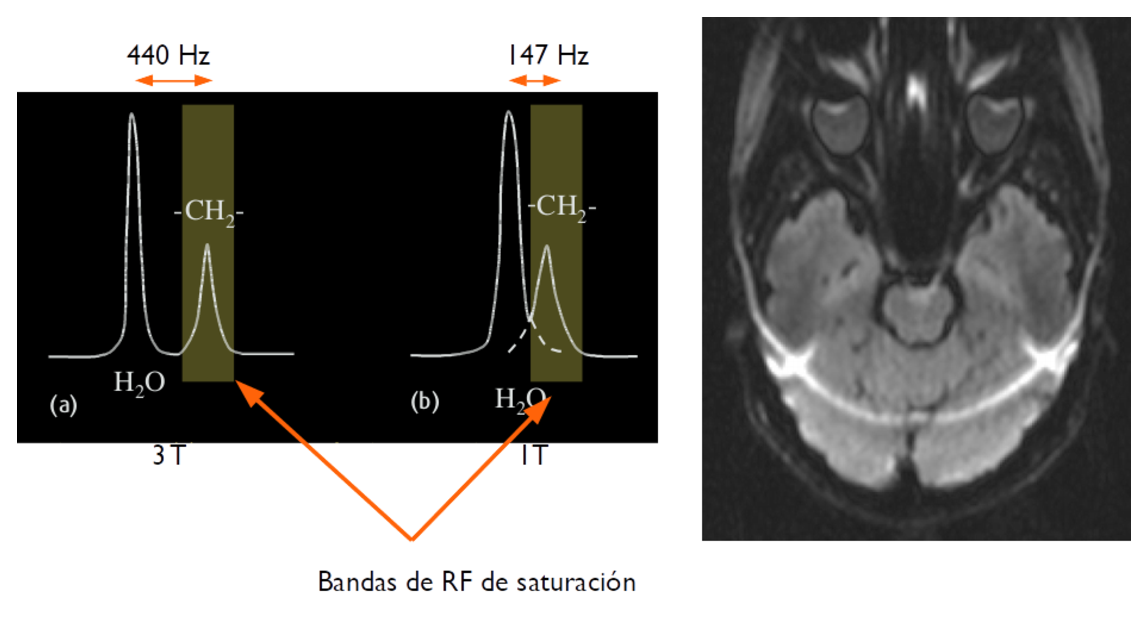
\includegraphics[width=0.7\textwidth]{artefacto_chemicalshift1}
   \caption{\figurapendiente}
 \label{fig:artefacto_chemicalshift1}
 \end{figg}
\end{figure}



\subsubsection{Artefacto por corrimiento químico Tipo 2}
La diferencia entre las precesiones de los protones asociados a \ce{H2O} y grasa es constante (3.5 ppm). Justo después de un pulso de RF excitador, los spins del agua y la grasa estarán precesando en fase, pero conforme pase el tiempo, se comenzarán a desfasar. La diferencia constante entre sus precesiones hará que en ciertos momentos predecibles las fases de los \ce{H} del agua y la grasa estén alineadas, y en otros momentos (también predecibles) estén perfectamente separadas por 180\degrees. Usando la analogía de los corredores en una pista de atletismo, donde uno es ligeramente más veloz que el otro, podemos imaginar que, en una carrera larga, habrá momentos en que ambos corredores estén alineados (al iniciar la carrera y cada vez que el corredor veloz logre avanzar por una vuelta completa a su lento adversario), mientras que habrá momentos en que el corredor veloz tenga r exactamente media vuelta de por medio entre él y su rival. En términos de la señal de resonancia que se produce, los momentos en que las fases de grasa y agua estén en fase provocarán interferencia constructiva, aumentando la amplitud de la señal recibida; cuando estén con fases distintas (a 180\degrees entre sí), la interferencia será desctructiva, y la cancelación entre las dos frecuencias harán que se pierda señal (Figura \ref{fig:artefacto_chemicalshift2}). Este artefacto no sucede en imágenes por eco de spin, ya que el pulso RF de 180\degrees vuelve a alinear las fases entre agua y grasa. 



\begin{figure}[htb]
 \begin{figg}
   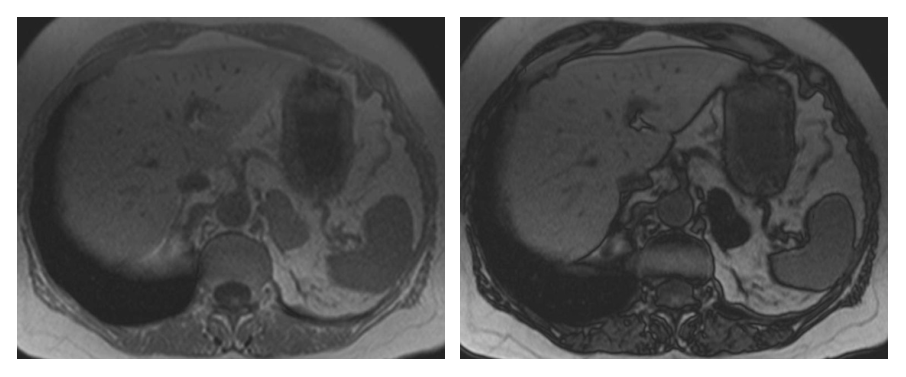
\includegraphics[width=0.7\textwidth]{artefacto_chemicalshift2}
   \caption{\figurapendiente Tomado de \url{https://radiologykey.com/shift-type-2-artifact/}}
 \label{fig:artefacto_chemicalshift2}
 \end{figg}
\end{figure}

Es fácil predecir en qué momento tendremos spins en fase o no, basándonos en $\Delta f$. Dado que $periodo = 1/f$, podemos predecir que habrá coincidencia de fases cada $1/\Delta f$. En un resonador de 1.5 teslas, esto es cada 1/224 Hz =  4.4 ms. Por consiguiente, las fases estarán en fase justo después del pulso RF excitador y cada 4.4 ms ([0 4.4 8.8 \ldots]), y a 180\degrees entre ellas a los 2.2 ms, y cada 4.4 ms después ([2.2 6.6 11.0 \ldots]). De esta forma, seleccionando un TE determinado, el usuario puede obtener una imagen dentro o fuera de fase. Cuando están fuera de fase, por ejemplo, las estructuras con recubrimiento graso tendrán una apariencia hipointensa que remarca sus bordes en la imagen.

Este artefacto puede utilizarse a favor para lograr imágenes que contienen de manera selectiva la señal del agua o de la grasa, con base en álgebra muy sencilla. Dado que las imágenes ($I$) dentro/fuera de fase tienen la siguiente relación:

\begin{equation*}
 \begin{aligned}
I_{dentro} = I_{agua} + I_{grasa} \\
I_{fuera} = I_{agua} - I_{grasa}
  \end{aligned}
\end{equation*}
se obtiene que
\begin{equation*}
 \begin{aligned}
I_{dentro} + I_{fuera} = 2 \times I_{agua} \\
I_{dentro} - I_{fuera} = 2 \times I_{grasa}
 \end{aligned}
\end{equation*}

Esta estrategia se conoce como el método de Dixon \cite{dixon1984} y es útil en la clínica y la investigación. \footnote{Visita \url{http://xrayphysics.com/chem_sh.html} para un simulador del método de Dixon.}



\subsection{Efecto dieléctrico}
Las ondas de RF interactúan con el medio. Las ondas de la red inalámbrica de internet en casa, por ejemplo, rebota en los muros y ocasiona sitios donde su amplitud es baja. El tejido también es capaz de reflejar y provocar refracción de ondas de RF emitidas por la antena transmisora del resonador, a la vez que las mismas ondas RF interactúan eléctricamente con el tejido. En el artefacto por efectos dieléctricos se aglomeran todos aquellos que son causados por interacciones entre la RF y el tejido. Estos efectos son prácticamente imperceptibles en resonadores de bajo campo magnético (menores a 1.5 T), pero son más evidentes conforme \Bzero aumenta. Esto se debe a que la longitud de onda de la RF es inversamente proporcional a su frecuencia (y, por lo tanto, a \Bzero). En un resonador de 3 teslas, por ejemplo, la longitud de onda de RF ($\lambda$) es de 26 cm, que es aproximadamente la dimensión del FOV habitual en humanos. El valle y la cresta de una onda de RF con esta longitud de onda estarían representadas a lo largo de la imagen, con lo que pueden producirse, por ejemplo, inhomogeneidades severas de excitación (Figura \ref{fig:artefacto_dielectrico}). En la medida en que aumenta la disponibilidad de resonadores de muy alto campo magnético (7 teslas o más; $\lambda$ = 11 cm) este artefacto cobrará mayor relevancia. 


\begin{figure}[htb]
 \begin{figg}
   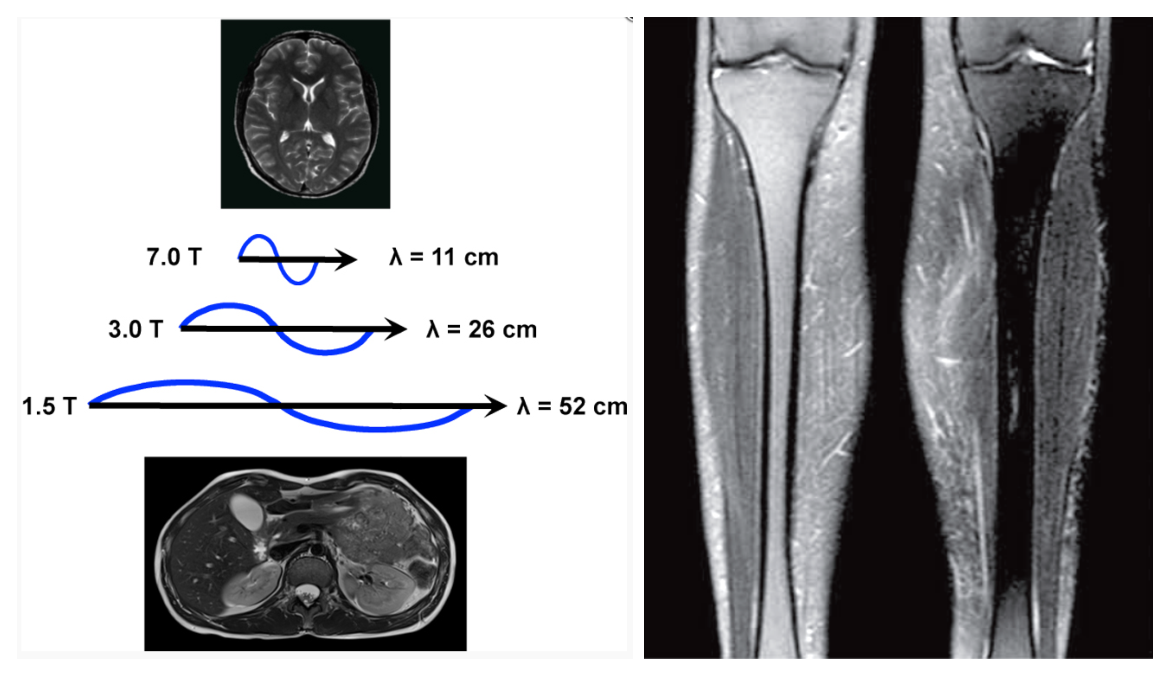
\includegraphics[width=0.7\textwidth]{artefacto_dielectrico}
   \caption{\figurapendiente}
 \label{fig:artefacto_dielectrico}
 \end{figg}
\end{figure}

